% !TEX TS-program = pdflatexmk


\documentclass[11pt]{report}

\usepackage[
%	notes,
	backend=biber,
%	isbn=false,
%	annotation,
%	notetype=endonly
	]{biblatex}
\DeclareFieldFormat{addendum}{\paragraph\indent{\textbf{Suggestions for Future Research:}\addspace#1}\\}\DeclareFieldFormat{annotation}{\paragraph\indent{\textbf{Brad's Notes:}\addspace#1}\\}
\DeclareFieldFormat{institution}{\paragraph\indent{\textbf{Institution:}\addspace#1}\\}


\usepackage{tikz}
\usetikzlibrary{arrows}
\usetikzlibrary{shapes}
\usetikzlibrary{patterns}
\usetikzlibrary{positioning}
\usetikzlibrary{decorations.pathmorphing}
%\usetikzlibrary{patterns,positioning,decorations.pathmorphing,arrows,shapes
\usetikzlibrary{fit}

\usepackage{pgfmath}
\usepackage[edges]{forest}

\usepackage{setspace}
\usepackage{amsmath}
\usepackage{amsthm}
	\newtheorem*{theorem}{Theorem}
	\newtheorem*{lemma}{Lemma}
	\newtheorem*{definition}{Definition}
\usepackage{amssymb}

\usepackage{array}
\usepackage{multirow}

\usepackage{hyperref}
\usepackage{enumerate}
\usepackage{enumitem}
\setlist{noitemsep}

\usepackage{listings}
\lstset{language=C}

\usepackage{makeidx}
\usepackage{verbatim}
\usepackage{datetime}

\setcounter{tocdepth}{2}

\setlength{\pdfpageheight}{11in}
\setlength{\textheight}{9in}
\setlength{\voffset}{-1in}
\setlength{\oddsidemargin}{0pt}
\setlength{\marginparsep}{0pt}
\setlength{\marginparwidth}{0pt}
\setlength{\marginparpush}{0pt}
\setlength{\textwidth}{6.5in}


\def\sinline[#1]{ \ \tikz\draw[decorate,decoration={snake,amplitude=0.6mm, segment length=14pt},->] (0,0) -- (.6,0) node [midway, above] {#1}; \ }

\pagestyle{plain}
\makeindex

\title{Literature Review for Imbalanced Data}
\author{Brad Burkman}
\newdateformat{vardate}{\THEDAY\ \monthname[\THEMONTH]\ \THEYEAR}
\vardate
\date{\today}

\addbibresource{../Papers/BibFile_Spring_2022.bib}

\begin{document}
\setlength{\parindent}{20pt}
\begin{spacing}{1.2}
\maketitle
\tableofcontents

%%%%%%%%%%%%%%%%%%
% Index
% Example of how to put something in the index:
% This item will be listed as "Definition" under the heading of "Articulation Node."
%		\index{Articulation Node!Definition}

\newpage
\phantomsection
\addcontentsline{toc}{chapter}{Index}
\printindex


%%%%%%%%%%
\chapter{To Do}

%%%%%
\section{Topics Remaining}

\subsection{Big Items}

\begin{itemize}
	\item Crash Analysis Lit Review
	\item Data Overview and Analysis
	\item Research Plan
\end{itemize}

\subsection{Details}
\begin{itemize}
	\item Worked through Brad's Reports
	\item Find where it mentions multiple Tomek runs.  
	\item Work through this tutorial, which will explain Condensed Nearest Neighbor.
	
	https://machinelearningmastery.com/undersampling-algorithms-for-imbalanced-classification/
	
	\item Figure out what Rough Sets Theory and Fuzzy Sets are.  
	\item Learn to use ROC curves.
	\item Review different types of models and how to implement them in Keras.
	\item Bagging and Boosting
	\item Topological Data Analysis
	
	Giotto-tda is a Python package dedicated to integrating TDA in the machine learning workflow by means of a scikit-learn API

\end{itemize}

%%%%
\section{Plan}

\begin{itemize}
	\item Identify review papers by established experts that give overviews of the field.  Use these as a ``textbook'' for imbalanced data.
	\item Write a review of the field (similar to my study guide for the Algorithms Comp)
	\begin{itemize}
		\item Topics
		\begin{itemize}
			\item Benchmark datasets for imbalanced classification.
			\item Sampling methods
			\item Metrics
			\item Loss functions
			\item Bagging and Boosting
			\item Math and CS tools, like Principal Component Analysis
		\end{itemize}
		\item For each topic
		\begin{itemize}
			\item Original and significant papers
			\item Theory and rationale
			\item Examples of usage in the field
			\item Example where I implement it
			\item If appropriate, implement it on the crash data
		\end{itemize}

	\end{itemize}
\end{itemize}

%%%%%
\section{Paper Standards}

When I took a 619 with Dr. Raghavan, he rejected my first draft of my paper because it could be summarized as, ``I used existing methods to do the same thing other people have done, but on my own data.''  He expected me to have done more thinking and synthesis.  

I had written the paper that way because that's what most of the papers I'd read did.  I learned later that I had been reading in a low-ranked journal.  

I feel like most of the {\it Accident Analysis and Prevention} papers are like that, ``I did a thing!''  If this field had benchmark datasets, it would be easier to see what is actually new in each article.  The {\it AAP} journal is not well ranked.  The {\it Transportation Research: Part C, Emerging Technologies} is better in both content and rankings.  I'll use the {\it TRC} articles as models.

%%%%%
\section{Paper Outline Idea from 7/19/21 Report}

\begin{enumerate}
	\item Louisiana Crash Dataset and its Challenges
	\begin{enumerate}[label=\alph*.]
		\item General Description
		\item Some data is missing
		\item Some data is unreliable or obviously wrong
		\item Data is imbalanced
	\end{enumerate}
	\item Incorporating Other Data
	\begin{enumerate}[label=\alph*.]
		\item Weather
		\item Urban/Rural
	\end{enumerate}
	
	\item Data Cleanup:  Methods
	\begin{enumerate}[label=\alph*.]
		\item Comparison of methods for handling missing data
		\item Methods for dealing with outliers
	\end{enumerate}
	\item Features:  Methods
	\begin{enumerate}[label=\alph*.]
		\item Engineering New Features
		\item Selecting Features [Incorporate Jing Chen's methods]
	\end{enumerate}
	\item Imbalanced Data:  Comparison of Methods
	\begin{enumerate}[label=\alph*.]
		\item Oversampling
		\item Understampling
		\item \verb|class_weight = 'balanced'|
		\item Finding balance between methods [pun intended]
	\end{enumerate}
	\item New Metrics: {\it Balanced Precision} and {\it Balanced f1}
	\begin{enumerate}[label=\alph*.]
		\item Definitions
		\item Justification
		\item Examples
	\end{enumerate}
	\item Models
	\item Balancing Everything
	\item Conclusion
	
\end{enumerate}
 



\chapter{Methods}

%%%%%
\section{Algorithm Level Approaches}
\index{Algorithm Level Approaches}

%%%
\subsection{Some Papers}
\begin{itemize}
	\item Recognition-based:  Learning from one class rather than discrimination-based, doing unsupervised learning on the minority class. \cite{CHAWLA_2004}
	\item Fuzzy rule-based classification systems (what is this?)
		\cite{CHABBOUH_2019} 
		\cite{DABLAIN_2021}
		\cite{MAHMUDAH_2021} 
		\cite{ZHAI_2020} 
		\cite{ZHAI_2020_D2GAN}
	\item In decision trees, using evolutionary/genetic methods instead of greedy search 
		\cite{CHABBOUH_2019} 
		\cite{WEISS_2000}
	\item Clustering and Subspace Modeling \cite{CHEN_2011}
\end{itemize}

%%%
\subsection{Genetic Algorithms}
\index{Genetic Algorithms}

In this short 2000 paper, Weiss \cite{WEISS_2000} used a genetic algorithm to predict rare events. Borrowing from simulated annealing, they varied the relative importance of precision and recall at each step of the genetic algorithm.  

%%%
\subsection{Subspace Model}
\index{Subspace Model}

Chen 2011 \cite{CHEN_2011}

This was fascinating and entirely different from anything I've seen.  

\begin{enumerate}
	\item Separate the training data $Tr$ into negative (majority) and positive (minority) classes $TrN$ and $TrP$.
	\item Let $K$ be the ratio of negative to positive samples, in my case about 100, so that if you divide the majority class $TrN$ into $K$ groups, each will have about the same number of samples as the minority class.
	\item Use $K$-means clustering to separate the negative (majority) class $TrN$ into $K$ groups; each of the groups is a cluster of the negative (majority) class.
	\item For each of the $K$ groups $TrN_i$:
	\begin{itemize}
		\item Combine the negative elements of the group with the entire positive (minority) class $TrP$ to form a balanced subspace.  
		\item Train the model for the subspace
	\end{itemize}
	\item Recombine the $K$ subspace models with a model trained on the entire data set to build an integrated model.
\end{enumerate}


%%%%%
\section{Loss Functions}

%%%%%
\subsection{Binary Cross-Entropy Loss Function}
\index{Binary Cross-Entropy}

Let's say we have an imbalanced data set with 100 negative samples for each positive sample.  

For binary classification, the first three (class weights, weighted loss function, and na\"{i}ve oversampling) are effectively the same in the training phase.  The cross-entropy loss function, 

$$loss = \sum_{i=1}^n y_i \log(p_i) + (1-y_i) \log (1-p_i)$$

for binary classification is

$$loss = \sum_{y_i=1} \log (p_i) + \sum_{y_i=0} \log (1-p_i)$$

which is the sum of the logs of the errors in predictions for the negative class plus the sum of the logs of the errors in predictions for the positive class.  

%%%
\subsection{Class Weights and $\alpha$-weighted Loss}
\index{Class Weights}
\index{$\alpha$-Weighted Loss}

If the classes are imbalanced, like there are 100 times as many samples with $y=0$ as samples with $y=1$, then the loss function is mostly summing how bad the predicting probability is for the majority class and largely ignoring the minority class.  Both the class weights parameter and a weighted loss function fix this by multiplying one or the other by some compensating factor.

$$loss = 100 \times \sum_{y_i=1} \log (p_i) +  \sum_{y_i=0} \log (1-p_i)$$

This multiple gives the two classes equal weight in the loss.  

In the $\alpha$-weighted cross entropy, 

$$loss = \sum_{i=1}^n \alpha y_i \log(p_i) + (1 - \alpha) (1-y_i) \log (1 - p_i)$$

let $\alpha = \frac{100}{100+1}$ and you'll get the same thing, within a positive constant multiple.  

$$loss = \sum_{i=1}^n \frac{100}{101} y_i \log(p_i) + \frac{1}{101} (1-y_i) \log (1 - p_i)$$

$$loss = \frac{1}{101}\sum_{i=1}^n 100 y_i \log(p_i) + (1-y_i) \log (1 - p_i)$$

The only difference I can ascertain between the class weights parameter and a weighted loss function is that the class weights aren't used with the validation set.  

%%%
\subsection{Oversampling}
\subsection{Na\"{i}ve Oversampling}
\index{Oversampling (Random)}

Na\"{i}ve oversampling would be to create 99 copies of each of the positive samples, so that the two sets are balanced.  That would have exactly the same effect on the loss function, because there would now be 100 times as many samples with $y_i=1$.  

%%%%%
\subsection{Class Weights v/s Na\"{i}ve Oversampling: They're the Same}

I had an insight on why these things are the same.  Let's say you have an imbalanced data set, with 100 times as many negative samples as positive samples.  

In Na\"{i}ve Oversampling, you make 100 copies of each of the positive samples and run regular cross-entropy loss.  

In weighted Class Entropy, you multiply the positive-class losses by 100.

$$loss = 100 \times \sum_{y_i=1} \log (p_i) +  \sum_{y_i=0} \log (1-p_i)$$

These two approaches different in execution but the same in result because, as I often remind my students, multiplying something by 100 is the same as adding it to itself 100 times.  



%%%
\subsection{Focal Loss}
\index{Focal Loss}

Introduced by Lin in 2017.  \cite{LIN_2020}

Yu 2020 \cite{YU_2020} adapts $\alpha$-weighted cross entropy and focal loss to crash analysis.


In the focal loss function, 

\begin{align*}
	loss &= \sum_{i=1}^n \alpha (1 - p_i) ^{\gamma_1} y_i \log (p_i) + (1 - \alpha) p_i^{\gamma_2} (1 - y_i)  \log (1 - p_i) \cr
	loss &= \sum_{y_i=1} \alpha (1 - p_i) ^{\gamma_1} \log (p_i) + \sum_{y_i=0} (1 - \alpha) p_i^{\gamma_2}   \log (1 - p_i) \cr
	\end{align*}

if $\gamma_1= \gamma_2 = 0$, then it's the same as the $\alpha$-weighted loss function.  

In the original focal loss paper by Lin \cite{LIN_2020}, $\gamma_1$ and $\gamma_2$ are the same.  

For samples with $y_i=1$, the minority class, here are values of $(1 - p_i) ^{\gamma_1} \log (p_i)$ for different values of $p_i$ and different values of $\gamma_1$.  I got the range of values of $\gamma_1 \in \{0, 0.5, 1, 2, 5\}$ from Lin's 2018 paper  that proposed focal loss.  

\begin{center}
\begin{tabular}{rl | llllll}
	&& \multicolumn{5}{c}{$\gamma_1$} \cr
	$(1 - p_i) ^{\gamma_1} \log (p_i)$ & & 0 & 0.5 & 1 & 2 & 5 \cr \hline
	& 0.1 & -3.32 & -3.15 & -2.99 & -2.69 & -1.96 \cr
	& 0.3 & -1.74 & -1.45 & -1.22 & -0.85 & -0.29 \cr
	$p_i$ & 0.5 & -1 & -0.71 & -0.5 & -0.25 & -0.03 \cr
	& 0.7 & -0.51 & -0.28 & -0.15 & -0.05 & 0 \cr
	& 0.9 & -0.15 & -0.05 & -0.02 & 0 & 0 \cr\end{tabular}
\end{center}

If $\gamma_1 > 0$, then for samples in the positive class, the loss is negligible for good predictions ($p_i$ close to 1), so it focuses the loss on poor predictions.  

Yu applied focal loss in the crash literature.\cite{YU_2020}

%%%
\subsection{Optimizing $F_\beta$}
\index{$F_\beta$}

Loss functions for gradient-based learning need to be differentiable (?), and the $F_\beta$ score is not differentiable, so this 2021 article by Lee \cite{LEE_2021} proposes a differentiable surrogate loss function that optimizes the $F_\beta$ score.  

With imbalanced data, using a loss function that optimized $F_\beta$ instead of accuracy would let you balance precision and recall, fixing one aspect of the imbalance problem.  

$$F_\beta = \frac{(1+\beta^2) \cdot \text{Precision} \cdot \text{Recall}}{(\beta^2 \cdot \text{Precision}) + \text{Recall}} 
= \frac{1}{
	\displaystyle\frac{\lambda_\beta}{\text{Recall}} + \frac{1 - \lambda_\beta}{\text{Precision}}
	}, 
	\qquad
	\lambda_\beta = \frac{\beta^2}{1 + \beta^2}
$$

The article takes a deep dive into loss functions.  I should master it.  


%%%
\subsection{Tree-Based Methods}
\index{Tree-Based Methods}


Pendault \cite{PEDNAULT_2000} has a 2000 article on insurance risk modeling that incorporates ``a domain-specific optimization criterion... to identify suitable splits during tree building.''  It assigns different weights to {\it claim} and {\it nonclaim} records.  Because that strategy helps but does not entirely solve the imbalanced data problem, they also have a split criterion that prevents splits of really small branches, ``splinter groups,'' that are unlikely to contain any elements of the minority class because the minority class is so sparse.  


%%%%%
\subsection{$\alpha$-weighted Binary Cross-Entropy Loss Function as Ethical Tradeoff}
\index{Ethical Tradeoff}
\label{sec:Ethical_Tradeoff}

From \verb|Brads_Report_10_25_21|

I made a [perhaps paper-worthy?] connection between the loss function I want and the $\alpha$-weighted binary cross-entropy loss function, which is widely known and widely implemented, but, according to Yu's paper, not before used in crash-related modeling.  

\subsubsection{Matrix}

\hfil\begin{tabular}{r|c|c|c|}
	& Do Not &  \cr
	& Send & Send \cr
	& Ambulance & Ambulance \cr
	& $h_\theta(x_i)<0.5$ & $h_\theta(x_i)>0.5$  \cr\hline
	Do Not Need Ambulance \  $y_i=0$ & TN & FP \cr \hline
	Need Ambulance \   $y_i=1$ & FN & TP \cr\hline
\end{tabular}

\subsubsection{Switching between Binary and Continuous}

In the binary cross-entropy loss function, 

$$J = -\sum_{i=1}^N y_i \log( h_\theta (x_i)) + (1-y_i) \log( 1 - h_\theta (x_i))$$

the $y_i$ are binary, $y_i \in \{0,1\}$, but the model predictions, $h_\theta (x_i)$, are a probability, $h_\theta(x_i) \in (0,1)$.  


\

If we treat the model predictions as binary, replacing 

$$
\log ( h_\theta(x_i)) \to 
\begin{cases}
	0 & \text{if } h_\theta(x_i) <= 0.5 \cr
	1 & \text{if } h_\theta(x_i) > 0.5 \cr
\end{cases}
$$

and

$$
\log ( 1 -  h_\theta(x_i)) \to 
\begin{cases}
	0 & \text{if } 1 - h_\theta(x_i) <= 0.5 \cr
	1 & \text{if } 1 - h_\theta(x_i) > 0.5 \cr
\end{cases}
$$

then 

$$ TP = \sum_{i=1}^N y_i \log( h_\theta (x_i))$$

$$ TN = \sum_{i=1}^N  (1-y_i) \log( 1 - h_\theta (x_i))$$

and the loss function becomes $J = -(TP+TN)$

Why do we use the continuous instead of the binary in the loss function?  Because we want the predictions to be robust, so that when we use the model on unseen data, we can be more certain that it will correctly classify new instances.  The binary, however, are much easier to explain to non-technical people, or even technical people in other fields.  

%%%
\subsubsection{Scenario}

The medical ethicists and politicians decide on a number, $p$, such that we are willing to automatically dispatch $p$ ambulances when they aren't needed in order to send one ambulance when it is needed.   We want $$ \frac{\Delta FP}{\Delta TP} \le p$$

%%%
\subsubsection{Binary $h_\theta$}

Our loss function is $$FP - p\cdot TP $$

%%%
\subsubsection{Continuous $h_\theta$}

Use the $\alpha$-weighted cross-entropy loss function, as in Yu's paper and widely available.

$$J = -\sum_{i=1}^N \alpha y_i \log( h_\theta (x_i)) + (1-\alpha)(1-y_i) \log( 1 - h_\theta (x_i)), \quad \alpha = \frac{p}{p+1}$$

%%%
\subsubsection{Why are these equivalent?}

Adding a constant to the loss function, or multiplying it by a positive constant, does not change its effect.  

$FP - p \cdot TP$ is equivalent to $FP - p \cdot TP + (TN+FP)$, because $TN+FP$ is constant, so 
$FP - p \cdot TP$ is equivalent to $-(p \cdot TP+ TP)$.


$$FP - p \cdot TP$$
$$-(p \cdot TP + TN)$$
Multiplying by $\frac{1}{p+1}$ gives an equivalent loss function, because $\frac{1}{p+1}>0$.
$$-\frac{p \cdot TP + TN}{p+1}$$
$$- \left( \frac{p}{p+1} TP + \frac{1}{p+1} TN\right)$$
$$- \left( \frac{p}{p+1} TP + \left( 1 - \frac{p}{p+1} \right) TN \right)$$
$$- (\alpha TP + (1 - \alpha) TN) $$

The continuous version of $TP$ is 
$ \displaystyle \sum_{i=1}^N y_i \log( h_\theta (x_i))$

The continuous version of $TN$ is 
$ \displaystyle \sum_{i=1}^N (1-y_i) \log( 1 - h_\theta (x_i))$

$$J = -\sum_{i=1}^N \alpha y_i \log( h_\theta (x_i)) + (1-\alpha)(1-y_i) \log( 1 - h_\theta (x_i)), \quad \alpha = \frac{p}{p+1}$$

%%%
\subsubsection{Emphasis in Our Work}

Yu et al introduced to the crash-analysis field the alpha-weighted cross-entropy loss function to deal with imbalanced data.  We propose another application of the alpha-weighted loss, to encode and implement tradeoffs that come from our ethical/political values decided by community leaders.   



%%%%%
\section{Data Level Methods}

%%%
\subsection{Imbalanced Cleaning:  Tomek and Condensed Nearest Neighbor}
\index{Tomek Links}
\index{Condensed Nearest Neighbor}

Batista
\cite{BATISTA_2004}
uses two imbalanced cleaning method called {\it Tomek links} and {\it Condensed Nearest Neighbor}.  If examples from the majority and minority class are close to each other, it deletes the majority samples.   One could think of it as targeted undersampling of the majority set.  

Imbalanced-Learn, an add-on to Scikit-Learn, has these algorithms read to use.  Tomek and Wilson's papers introducing these algorithms are from the 1970's.  
\index{Imbalanced-Learn}


%%%
\subsection{Tomek's Links}

This method undersamples the majority-class samples, eliminating ones that are too close to minority-class samples, presuming them to be noise, and helping clarify clusters of minority samples.  

A pair of samples are a {\it Tomek link} if one is majority and one minority, and they are each other's nearest neighbors. To use Tomek's inks as an undersampling strategy for imbalanced data, delete the positive sample in each Tomek's link.  Other cleaning strategies (for balanced sets) would eliminate both the positive and negative.  

It is possible to iterate Tomek's several times.  Here's an example of how it works in one round and in a second round.  The blue samples are from the majority set and the red are from the minority.  Assume that these seven points are a small part of a large dataset, but these are the only points in this region.

\

\noindent\hfil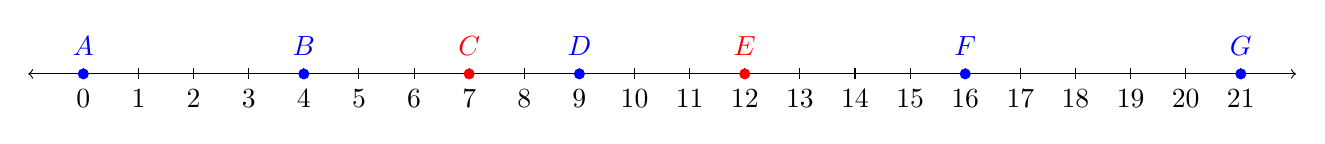
\begin{tikzpicture}[x=7mm, y=7mm]
	\draw [<->] (-1,0) -- (22,0);
	\foreach \x in {0,1,2,...,21}
		\draw (\x, 0.1) -- (\x,-0.1) node [below] {$\x$};
	\fill [blue] (0,0) circle (2pt) node [above=3pt, blue] {$A$};
	\fill [blue] (4,0) circle (2pt) node [above=3pt, blue] {$B$};
	\fill [blue] (9,0) circle (2pt) node [above=3pt, blue] {$D$};
	\fill [blue] (16,0) circle (2pt) node [above=3pt, blue] {$F$};
	\fill [blue] (21,0) circle (2pt) node [above=3pt, blue] {$G$};
	\fill [red] (7,0) circle (2pt) node [above=3pt, red] {$C$};
	\fill [red] (12,0) circle (2pt) node [above=3pt, red] {$E$};
\end{tikzpicture}

In the original dataset, $C$ and $D$ are each other's nearest neighbors, $C$ from minority and $D$ from majority, so they are a Tomek link.   On the other hand, $D$ is the nearest neighbor to $E$, but $E$ is not $D$'s nearest neighbor, so they are not a Tomek link.  

Eliminate sample $D$.  

\

\noindent\hfil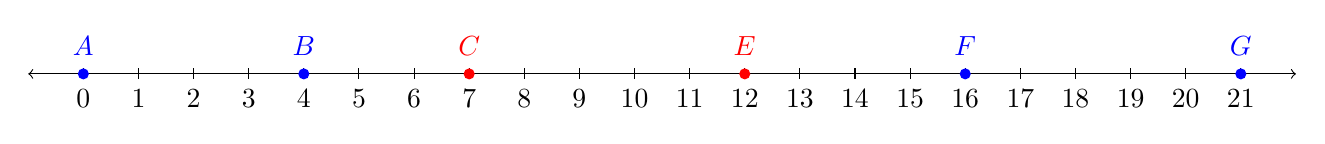
\begin{tikzpicture}[x=7mm, y=7mm]
	\draw [<->] (-1,0) -- (22,0);
	\foreach \x in {0,1,2,...,21}
		\draw (\x, 0.1) -- (\x,-0.1) node [below] {$\x$};
	\fill [blue] (0,0) circle (2pt) node [above=3pt, blue] {$A$};
	\fill [blue] (4,0) circle (2pt) node [above=3pt, blue] {$B$};
%	\fill [blue] (9,0) circle (2pt) node [above=3pt, blue] {$D$};
	\fill [blue] (16,0) circle (2pt) node [above=3pt, blue] {$F$};
	\fill [blue] (21,0) circle (2pt) node [above=3pt, blue] {$G$};
	\fill [red] (7,0) circle (2pt) node [above=3pt, red] {$C$};
	\fill [red] (12,0) circle (2pt) node [above=3pt, red] {$E$};
\end{tikzpicture}

Now the pairs $(B,C)$ and $(E,F)$ are Tomek links, so if we ran Tomek undersampling a second time, we would remove samples $B$ and $F$.  

\

\noindent\hfil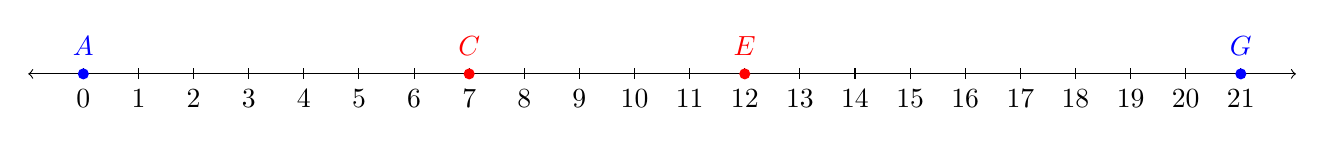
\begin{tikzpicture}[x=7mm, y=7mm]
	\draw [<->] (-1,0) -- (22,0);
	\foreach \x in {0,1,2,...,21}
		\draw (\x, 0.1) -- (\x,-0.1) node [below] {$\x$};
	\fill [blue] (0,0) circle (2pt) node [above=3pt, blue] {$A$};
%	\fill [blue] (4,0) circle (2pt) node [above=3pt, blue] {$B$};
%	\fill [blue] (9,0) circle (2pt) node [above=3pt, blue] {$D$};
%	\fill [blue] (16,0) circle (2pt) node [above=3pt, blue] {$F$};
	\fill [blue] (21,0) circle (2pt) node [above=3pt, blue] {$G$};
	\fill [red] (7,0) circle (2pt) node [above=3pt, red] {$C$};
	\fill [red] (12,0) circle (2pt) node [above=3pt, red] {$E$};
\end{tikzpicture}

Now $C$ and $E$ are each other's nearest neighbors and of the same (minority) class, so this part of the dataset would not change under another run of Tomek.  

The idea of Tomek assumes that the minority samples should cluster, and any majority samples in or near those clusters must be noise, so we can eliminate them.  We now have a clear cluster of two minority samples with no close majority samples.  

I saw multiple runs of Tomek mentioned [somewhere] in my reading, so  I tried it on the crash data, running it up to five times, and saw that it converged, with fewer positive samples eliminated in each round.  I had conjectured that a negative sample in a Tomek link in a later round must have been a negative sample in a Tomek link in an earlier round, digging itself out of a field of positive-class dust, but I suspected that there might be (perhaps unusual) cases where one minority-class sample ($C$ in the example above) created a Tomek link, and eliminating the majority-class sample in that link ($D$ above) allowed a Tomek link for a different minority-class sample ($E$ above).  I then played with it until I found a counterexample to my conjecture, so the conjecture, that a minority-class sample in a Tomek link in a later round of Tomek undersampling must have been in a Tomek link in every previous round of the Tomek undersampling, is false.  

If the conjecture had been true, then we could greatly speed up subsequent rounds of Tomek undersampling by only considering the minority samples in Tomek links in the previous round.  That would not be thorough, but this approach would.  

\subsubsection{Algorithm for Repeated Application of Tomek's Links}

	For the first round of Tomek undersampling, one has to consider each element of the minority class.  In the Tomek's links, call the minority-class elements $\{A_{1}, A_{2}, \dots, A_{n1}\}$, and the majority-class elements $\{B_1, B_2, \dots, B_{n1}\}$.  Tomek undersampling for minority classes eliminates all of $\{B_1, B_2, \dots, B_{n1}\}$.
	
	In the second round of Tomek undersampling, we only need to consider as possible Tomek links the nearest neighbors of $\{A_{1}, A_{2}, \dots, A_{n1}\}$ and any element of the minority class that had one of $\{B_1, B_2, \dots, B_{n1}\}$ as its nearest neighbor.
	
In subsequent rounds, consider the minority-class samples from the Tomek's links from the previous round, and the elements of the minority class that had as their nearest neighbor an element of the majority class in the Tomek's links.  

In theory there could be more Tomek's links in one round than in the previous round, but in practice they go to zero and the set converges to a set with no Tomek's links.  

%%%
\subsection{Cleaning Multiclass Data}

Wei (2021) \cite{WEI_2021} uses something similar to Tomek's links for a multi-class problem with a majority class and multiple minority classes.  

\begin{itemize}
	\item Splits an imbalanced multi-class problem with $n+1$ classes ($n$ of them being minority) into $n$ imbalanced binary problems for data cleaning.  
	\item Uses cleaning undersampling (similar to Tomek's Links) to remove noisy spots in the data.
\end{itemize}


%%%
\subsection{Oversampling}

Naive oversampling would be to create 99 copies of each of the positive samples, so that the two sets are balanced.  That would have exactly the same effect on the loss function, because there would now be 100 times as many samples with $y_i=1$.  


%%%
\subsection{Underssampling}

Undersampling would erase 99\% of the negative samples so that the classes would be balanced.  That seems like a bad idea, because you would lose a lot of information about the majority class.  

\subsection{SMOTE:  Synthetic Minority Oversampling TEchnique}

Especially if we're doing fatalities, we have a terribly imbalanced data set.  Ideally we'd like to have an equal number of fatal and nonfatal crashes to plug into our ML algorithm, but we have about 0.47\% fatal and 99.53\% nonfatal.  

One solution is to randomly choose 681 nonfatal crashes to compare with our 681 fatal crashes, but that leaves behind a LOT of information.  

Many of the papers I've read use SMOTE, which balances the data set by creating synthetic elements for the minority set (fatal crashes).  It picks an element of the minority set, $a$, and picks one of its nearest neighbors, $b$, and creates a new synthetic element $c$.  For each data category, $D_i$, in which they differ, SMOTE chooses $D_i(c)$ to be between $D_i(a)$ and $D_i(b)$.  It randomly chooses a random number $r \in [0,1]$, and makes $D_i(c) = D_i(a) + r(D_i(a) - D_i(b))$.  

I get how that works for continuous variables.  I get that it would work if $D_i(a)$ and $D_i(b)$ weren't very different.  

How would that work for boolean variables?  SMOTE would choose nearest neighbors $a$ and $b$ that agree on most variables, but for values of $i$ where $D_i(a)=0$ and $D_i(b)=1$, it would randomly choose $D_i(c) \in \{0,1\}$.  There is no {\it between} for boolean variables.  It doesn't seem to me that it would work as well.  

Original SMOTE only works with continuous variables.  There is something called SMOTE-NC that handles continuous and categorical, but it has to have some continuous variables to work on.  

\begin{quote}
Unlike SMOTE, SMOTE-NC for dataset containing numerical and categorical features. However, it is not designed to work with only categorical features.
\end{quote}

\url{https://imbalanced-learn.org/dev/references/generated/imblearn.over_sampling.SMOTENC.html}

Since we have $\approx 200$ times as many nonfatal crashes as fatal crashes, to balance the data set with SMOTE, we would have to make two hundred synthetic elements for each fatal crash.  It seems to me that we would be making a mess of our data set.  
		


%%%
\subsection{Flavors of SMOTE}
\index{SMOTE}

SMOTE, or Synthetic Minority Oversampling TEchnique, 			\cite{CHAWLA_2002}
 creates extra samples of the minority class, but rather than making exact copies, it finds two similar samples and creates more samples ``between'' them, with feature values between the values of the two samples.  SMOTE only works for continuous features, not for categorical features.  Almost all of my features are categorical.  
 
 I got this list of flavors of SMOTE from a 2021 review by Mahmudah.
			\cite{MAHMUDAH_2021}  I've investigated some of them and given some flesh to some parts of this skeleton.
 
 		\begin{itemize}
			\item SMOTE:  Synthetic Minority Oversampling TEchnique 
			\cite{CHAWLA_2002}
			
			Uses $k$-nearest neighbors to find two close positive (minority) samples, and creates a synthetic sample between them.  Works on continuous data, not on categorical or binary data.  
			
			\item ADASYN:  ADAptive SYNthetic sampling approach for imbalanced learning.  
			\cite{MAHMUDAH_2021}
			
			Creates synthetic samples based on the level of difficulty in learning the samples of the minority class.  A positive samples is ``difficult'' if it has more negative samples as its nearest neighbors.  The more difficult a sample is, the more synthetic copies of that sample ADASYN creates.  
			
			\item Borderline SMOTE
			\cite{MAHMUDAH_2021}
			
			Generates synthetic positive samples along the border between the positive and negative classes.  Brad's Question:  This assumes you know where the border is.  I suppose you could do it iteratively.  
			
			\item Safe-level SMOTE
			\cite{MAHMUDAH_2021}

			When SMOTE finds the nearest positive-class neighbors of a positive sample, it ignores the negative (majority-class) neighbors.  [I think this is what it means:]  Creating synthetic positive-class samples in a neighborhood with lots of negative samples just makes more of a mess, so this is not considered a ``safe'' place to make synthetic samples.  Safe-level SMOTE creates synthetic positive samples only in majority-positive neighborhoods.  
			
			\item Relocating-safe-level SMOTE (RSLS)
			\cite{MAHMUDAH_2021}
			
			Avoids creating synthetic positive samples near negative samples.  
			
			\item Density-based SMOTE (DBSMOTE)
			\cite{MAHMUDAH_2021}

			Integration of DBSCAN and SMOTE.   DBSCAN, Density-Based Spatial Clustering of Application with Noise, discovers clusters with an arbitrary shape (?)  DGSMOTE creates synthetic samples at the pseudo-centroids of the clusters of positive samples.  
			
			\item Adaptive Neighbor SMOTE (ANS)
			\cite{MAHMUDAH_2021}

			Focuses not on -where- to generate synthetic samples, but on -how many- samples to generate in a particular neighborhood. 

			\item D2GAN 

This 2020 article by Zhai \cite{ZHAI_2020_D2GAN} builds on the Dual Discriminator Generative Adversarial Nets (D2GAN) paper from 2017 by Nguyen \cite{NGUYEN_2017}.  They want to do better oversampling, comparing D2GAN with SMOTE.  I don't understand what this is, but they say SMOTE has three drawbacks:

\begin{enumerate}
	\item Ignores the probability distribution of minority class samples.
	\item Synthetic examples lack diversity.
	\item Interating SMOTE many times will give synthetic samples with significant overlap.
\end{enumerate}

This 2022 article by Zhai \cite{ZHAI_2022} slightly modifies Zhai's claims against SMOTE.

\begin{enumerate}
	\item Does not extend the training field of positive samples.
	\item Synthetic examples lack diversity.
	\item Does not accurately approximate the probability distribution of minority class samples.
\end{enumerate}

The authors propose two new methods of diversity oversampling by generative models, one based on ``extreme machine learning autoencoder,'' and the other based on generative adversarial networks (GAN).  

			
		\end{itemize}
		

%%%
\subsection{Train/Test Split}

The application in Sharififar's 2019 article \cite{SHARIFIFAR_2019}  is digital mapping of farmland, categorizing areas by soil type.  Some soil types are rare but significant.  This is the first article I've seen that, at the beginning, says that making sure each minority class appears in appropriate distribution in the validation and test sets is an important challenge.  They explicitly say that they split 30\% for the validation set by taking 30\% of each class.

%%%
\subsection{Feature Selection}

This 2012 article by Tan \cite{TAN_2012} introduces a feature selection model specifically for imbalanced data sets.  I haven't dug in yet.  




%%%%%
\section{Bagging and Boosting}
\begin{itemize}
	\item Boosting and Bagging 
	\cite{BATISTA_2004} 
	\cite{CHABBOUH_2019} 
	\cite{DABLAIN_2021} 
	\cite{MAHMUDAH_2021} 
	\cite{SHARIFIFAR_2019}
\end{itemize}


%%%%%%%%%%
\chapter{Datasets}

\input{Datasets}


%%%%%%%%%%
\chapter{Interesting Papers}

%%%%%
\section{Review Papers}

%%%
\subsection{Chawla}
Chawla \cite{CHAWLA_2004} gives an overview of the state of the field in 2004.

\begin{itemize}
	\item Data Methods
	\begin{itemize}
		\item Random Oversampling with Replacement
		\item Random Oversampling
		\item Directed Oversampling
		
		No new examples are created, but the choice of which ones to replace is informed rather than random.
		\item Directed Undersampling
		\item Oversampling with informed generation of new samples
		\item Combinations of the above
	\end{itemize}
	\item Algorithmic Methods
	\begin{itemize}
		\item Adjusting class costs
		\item Adjusting the probabilistic estimate at the tree leaf (for tree methods)
		\item Recognition-based methods (learning from one class) rather than discrimination-based.
	\end{itemize}
	\item Issues at 2000 Conference
	\begin{itemize}
		\item 
	\end{itemize}
	\item Issues at 2003 ICML Conference
	\begin{itemize}
		\item Probabilistic estimates
		\item Pruning
		\item Threshold adjusting
		\item Cost-matrix adjusting.
	\end{itemize}
	\item Interesting Topics at 2003 ICML Conference
	\begin{itemize}
		\item Selective sampling based on query learning (Abe)
	\end{itemize}
	\item Overlapping Problems
	\begin{itemize}
		\item Class Imbalance
		\item Small Disjunct Problem (?)
		\item Rare Cases
		\item Data Duplication
		\item Overlapping Classes
	\end{itemize}
\end{itemize}

By 2003, the field started to mature.  


%%%
\subsection{Chabbouh 2019}

This article \cite{CHABBOUH_2019} has a nice table classifying existing work in imbalanced classification; however, I think much of the information was old in 2019, particularly C4.5, an early decision tree base classifier that may not be used much anymore.  


%%%
\subsection{Mahmudah 2021}

This article \cite{MAHMUDAH_2021} is really a review of current methods.   They have some datasets, most public benchmark sets, and throw every combination of tools at them. The ``methods'' section is really an overview of current methods.  

Has a section on techniques for feature extraction (feature engineering?) by dimensionality reduction, not particularly related to imbalanced data.  





%%%%%
\newpage
\phantomsection
\addcontentsline{toc}{chapter}{Bibliography}
\printbibliography



%%%%%%%%%%%%%%%%
\end{spacing}
\end{document}

%%%%%%%%%%%%
% Useful tools
%%%%%%%%%

\begin{lstlisting}
Put your code here.
\end{lstlisting}

\lstinputlisting[language=python]{source_filename.py}


